\section{Heurística Constructiva Golosa}

\subsection{Algoritmo}



\quad Analizando las características del problema implementamos una heurística constructiva golosa con los siguientes objetivos:

\quad

\quad \quad \quad - Empezar con el impacto máximo posible (cantidad de aristas de H)

\quad 

\quad \quad \quad - Modificar la menor cantidad de nodos posibles

\quad

\quad \quad \quad - El nodo que se modifique, tendría que bajar lo menos posible el impacto

\quad

\quad Pseudocódigo:

\begin{algorithm}[H]
\caption{} 
\begin{codebox}
\Procname{$\proc{maximoImpactoGoloso}(Grafo$ g$, Grafo$ h$, double porcentaje)$}

\li vector$<$unsigned int$>$ $res(n+1)$
\li int $solucion[0] \gets 0$
\li vector$<$unsigned int$>$ $coloreo(n,1)$
\li vector$<$bool$>$ $modificados(n,false)$
\li \While not G.coloreoLegal(coloreo)) \Do
\li nodo $ \gets $ siguienteModificable(G,H,modificados,porcentaje)
\li \For c desde 1 hasta colores.size() \Do
\li \If G.colorLegalDelNodo(nodo,coloreo,c)
\li coloreo$ [nodo] \gets $ c
\li exitFor
\End
\End
\End
\li $solucion[0] \gets$ impacto(h, coloreo)
\li \For i desde 0 hasta n \Do
		\li $solucion[i+1]=coloreo[i]$
	\End
\li	return $solucion$
\End
\end{codebox}
\end{algorithm}


\begin{algorithm}[H]
\caption{} 
\begin{codebox}
\Procname{$\proc{siguienteModificable}(Grafo$ g$, Grafo$ h,vector$<$bool$>$ modificados, double porcentaje)}

\li vector$<$pair$<$ unsigned int, unsigned int $>$ $>$ posibles
\li \For n nodo in V(G) \Do
\li \If not modificados$ [ $ nodo $ ] $
\li    agregar(posibles,$<$G.impactoNodo(nodo,H,coloreo),nodo$>$)
\End
\End
\li
\li sort(posibles)
\li
\li unsigned int res $ \gets $ random($ \vert $ posibles  $ \vert $ * porcentaje)
\li
\li return res
\End
\end{codebox}
\end{algorithm}

\quad

\quad En \textit{maximoImpactoGoloso} primero se colorea a todos los nodos con el mismo color, por lo que, sin tener en cuenta al grafo G, el impacto en H es máximo. Mientras que no sea legal este coloreo en G, se va a ir modificando los nodos. Apenas se consiga un coloreo legar se detiene. Por lo tanto, no necesariamente el ciclo principal itera la cantidad de nodos (en el peor caso sí).

\quad En \textit{siguienteModificable} se obtiene el nodo a modificar. Se crea una lista de nodos que no hayan sido modificados y se calcula para cada uno su aporte al impacto en H. Se ordena la lista por los siguientes criterios:

\quad

\quad \quad - Menor impacto en H aportado: se desea modificar al que menos aporta para ver si cambiando de color aporta más.

\quad

\quad \quad - Mayor grado en G: se busca que cuanto antes el coloreo de G sea legal modificando lo menos posible, y modificando un nodo de grado grande se podria conseguir esto.

\quad 

\quad \quad - Menor grado en H: por lo que dijimos, en caso de empate de los anteriores criterios, queremos modificar lo menos posible en G y H


\subsection{Análisis de complejidad}

\indent Comencemos analizando la complejidad de la función impactoNodo.\\
\indent Esta función mira para un nodo el impacto que aporta en H, comparando su color con el de sus vecinos. Dicho nodo tiene en H a lo sumo n-1 vecinos. Luego, impactoNodo cuesta O(n).

\indent Analicemos ahora siguienteModificable. Al inicio comienza iterando sobre la cantidad de nodos de H y si dicho nodo no fue modificado o si no tiene vecinos, se calcula el impacto de cada nodo y se lo agrega a un vector de nodos candidatos a ser modificados.En el peor caso, todos los nodos están sin modificar y tienen vecinos,por lo tanto esto cuesta O($n^{2}$).\\
\indent Luego, se ordena de manera creciente el vector de candidatos de acuerdo al impacto de cada nodo.En el peor caso dicho vector tiene n elementos, pues todos los nodos son modificables y ordenarlos cuesta entonces O(n*log(n)).\\
\indent Luego, se itera sobre la cantidad de elementos de ese vector, esta vez para desempatar los nodos. En el peor caso todos los nodos empatan en el impacto que generan. Desempatarlos a todos cuesta en el peor caso O($n^{2}$) , que el caso en el que se invirtió el orden del vector por desempates.\\
\indent A continuación se elige pseudoaleatoriamente en O(1) uno de los primeros elementos del vector.\\
\indent Pasando en limpio, siguienteModificable cuesta O($n^2$ + n*log(n)+ $n^2$), que es O($n^{2}$).\\

\indent Ahora analicemos maximoImpactoGoloso.\\
\indent Al principio realiza unas cuantas operaciones en O(n). De estas es destacable la creación de un vector de tamaño igual al grado del nodo con grado máximo de G, que refiere a la cantidad de colores a usar. Pero el grado máximo de cada nodo es a lo sumo n-1. Luego crear ese vector cuesta O(n).\\
\indent Luego, se ejecuta un while que a lo sumo itera n veces. Esto es porque en el peor caso tuve que pintar todos los nodos de distinto color hasta obtener un coloreo válido.\\
\indent Dentro de ese while está implícito el chequeo de si el coloreo es válido, que cuesta O(n+m), donde vamos a acotar a m como el máximo entre las aristas de G y de H. Se ejecuta siguienteModificable y se itera luego en la cantidad de colores, costando cada iteración en la cantidad de colores O(n) que es lo que cuesta ver si pintar un nodo de ese color es no coincide con el color de uno de los vecinos de ese nodo, que como mencionamos antes pueden ser n-1.\\
\indent Luego, lo de adentro del while cuesta O(n+m+ $n^{2}$) y el costo total del while es de O(n(n+m +$n^{2}$)), que es O(n*(n+m)+ $n^{3}$).\\
\indent Luego de iterar se calcula el impacto de dicho coloreo en O(n+m).\\
\indent Es decir que en total maximoImpactoGoloso cuesta O(n+n*(n+m)+ $n^{3}$ + n+m).\\
\indent Por lo tanto, maximoImpactoGoloso cuesta O(n*(n+m)+ $n^{3}$).\\
 
\subsection{Experimentación y Resultados}
\quad Trabajamos con los siguientes 3 casos: grafos al azar, grafos densos, G y H complementos.

\quad Se midieron los tiempos en corridas de  5 a 100 nodos con 100 repeticiones para cada cantidad de nodos.

\subsubsection{Grafos al azar}

\begin{figure}[H]
	\centering
	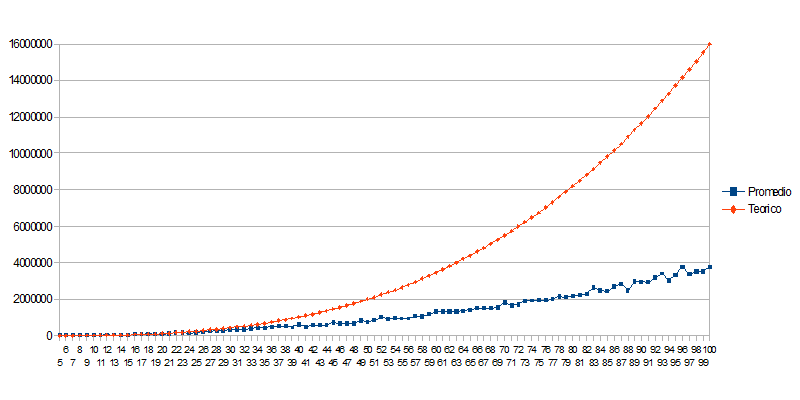
\includegraphics[scale=0.5]{goloso tiempos Azar.png}
\caption{Costos}
\end{figure}

\subsubsection{Grafos densos}

\begin{figure}[H]
	\centering
	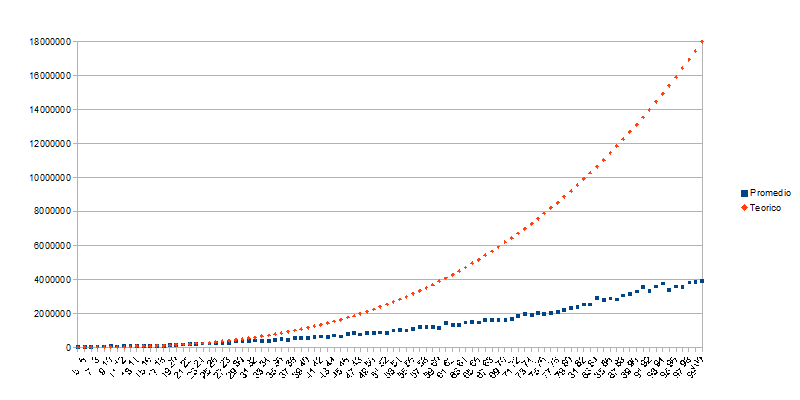
\includegraphics[scale=0.5]{goloso tiempos G y H densos.png}
\caption{Costos}
\end{figure}

\subsubsection{G y H complementos}

\begin{figure}[H]
	\centering
	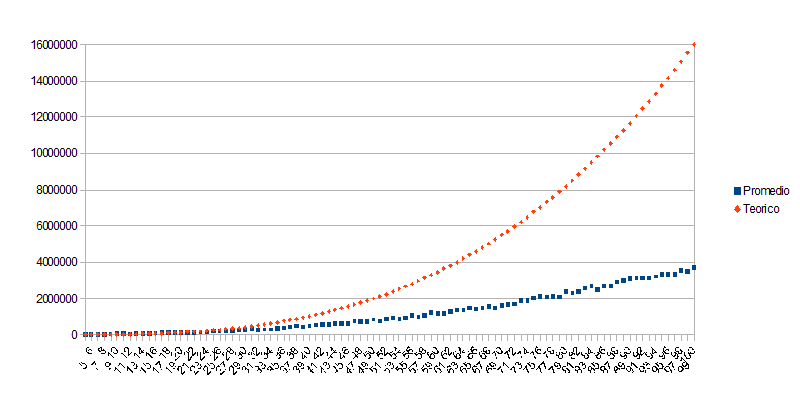
\includegraphics[scale=0.5]{goloso tiempos H complemento.png}
\caption{Costos}
\end{figure}